\section{Обзор существующих решений}
\label{sec:Chapter4} \index{Chapter4}

%В данной главе необходимо провести анализ существующих моделей. Аргументировать выбор тех или иных моделей, методов. Подготовить теоретическую базу перед экспериментов.


\subsection{Обзор моделей для распознавания КТ}
\label{sec:Chapter4_PE}

В данном разделе будут рассмотрены несколько моделей распознавания ключевых точек на теле человека. Некоторые из них довольно старые, но показывают неплохие результаты. Большинство же представлены не более 5 лет назад и являются лидерами направления на сегодняшний день.

\subsubsection*{DeepPose}

Данный представитель является самым старым решением из данной выборки и, одновременно, один из самых первых в целом. Статья "DeepPose: Human Pose Estimation via Deep Neural Networks"  \cite{DeepPose} была представлена исследователями из GOOGLE на конференции CVPR в 2014 году.

Исследователи разработали модель, представляющую сосбой каскад из DNN-регрессоров для локализации ключевых точек. Так как на тот момент не было выпущено общепринятых топологий, то в роли ключевых точек выступали суставы тела, а поза кодировалась их координатами, нормализованными на размер изображения.

\begin{figure}[h]
	\centering
	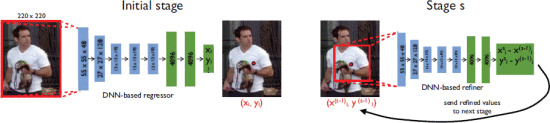
\includegraphics[width=\textwidth]{./images/DeepPose}
	\caption{Архитектура сети DeepPose. \cite{DeepPose}}
	\label{fig:dp_architecture}
\end{figure}

Работа модели делилась на два этапа, которые схематически показаны на \autoref{fig:dp_architecture}. На первом производилась локализация точки. Далее результаты переходили на второй этап, где пропускались через каскад из DNN, который производил уточнение предсказания. В результате получался отосительно точный результат, который можно было использовать для дальнейших исследований.

\subsubsection*{BlazePose}

Ахитектура BlazePose представлена в проекте MediaPipe

\subsubsection*{OpenPose}

OpenPose - это проект от лаборатории перцептивных вычислений университета Карнеги-Меллона в США. Проект включает в себя несколько моделей распознавания ключевых точек: на лице, руках, теле и различные их комбинации. Количество распознаваемых моделями точек доходит до 135 на одном человеке, а модель может распознавать сразу несколько человек на одном кадре. Скорость работы модели позволет использовать ее для распознавания видео в реальном времени через веб-камеру. К сожалению, основной репозиторий проекта не поддерживается с ноября 2020 года.

\begin{figure}[h]
	\centering
	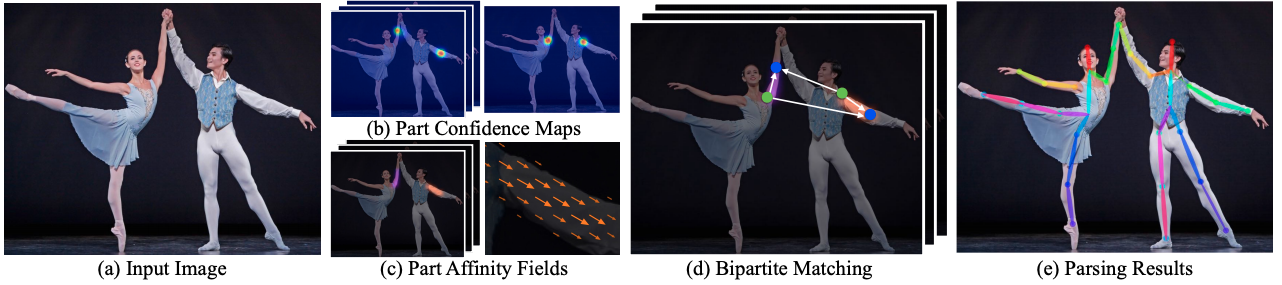
\includegraphics[width=\textwidth]{./images/OpenPose/structure}
	\caption{Последовательность распознавания ключевых точек моделью OpenPose. \cite{OpenPose}}
	\label{fig:op_structure}
\end{figure}

На данный момент обратимся к модели, резльтаты которой описываются тополгией из 25 точек. Данная модель одна из немногих в представленном обзоре, которая использует подход снизу вверх. Это достигается за счет использования двухступенчатой архитектуры нейросети (см \autoref{fig:op_structure}). 
 
В рамках первого этапа (вторая колонка на \autoref{fig:op_structure}) нейросетью предсказываются такие сущности, как карта достоверности обнаружения точки и карта двумарных векторных полей ориентации конечностей (англ. Part Affinity Fields или PAF). Изначально предсказание сущностей выполнялось паралельно, но взаимный анализ результатов предсказаний позволил увидеть возможность интуитивно предсказывать карты достоверности на основе PAFs. Это позволило значительно ускорить работу алгоритма.

Вторым этапом (треья колонка на \autoref{fig:op_structure}) происходит сопоставления точек и конечностей отдельным людям. Для увеличения точности и уменьшения времени построения скелетов используются графы соответсвия, которые позволяют создать целостные и непротиворечивые представления поз людей на изображении.

\subsubsection*{HRNet}

2019 год. Основная модель от проекта MMPose. Использует интересную архитектуру и хорошо показала себя при предыдущих сравнениях.

\subsubsection*{ViTPose}

Трансформер. ??? год. Интересная архитектура. Рассказать про трансформер, рассказать про кодеки/докедеки. Рассказать про способ работы. Можно расписатьсся неплохо.

\subsubsection*{RTMPose}

2023 год. На момент ислледования наиболее актуальная модель от проекта MMPose.

Работает неплохо. Обучается тоже неплохо. Попробуем заюзать в экспериментах.

\subsubsection*{Simcc + Resnet}

Вообще хз что это, но если смогу, то сделаю эксперимент )

\subsubsection*{YoloPose}

Несколько различных версий архитектуры Yolo дают несколько различных версий модели для распознавания позы. Использует подход снизу-вверх и хорошо


\subsection{Анализ и выбор методов доменной адаптации}
\label{sec:Chapter4_DA}

Опираясь на модели из предыдущей главы надо сделать анализ и выбрать только несколько методов, которые применимы к нашим требованиям и которые мы будем сравнивать между собой.

\subsubsection*{PUL}

Будем это использовать в работе. Надо будет хорошо расписать...

\subsubsection*{RegDA}

Интересный алгоритм. На нем базируются все остальные

\hfill \break

НАДО БУДЕТ ОСТАВИТЬ ТОЛЬКО ОДИН ИЗ СЛЕДУЮЩИХ МЕТОДОВ.

\subsubsection*{UDA PoseEstimation}

Адаптация от синтетических данных к реальным. Должно бтыь интересно описать. Не использовали, так как до сих пор мы не перешли в 3х мерное пространство.

\subsubsection*{POST}

Похожее на предыдущее

\subsubsection*{SFDA}

Похожее на предыдущее


\newpage
